%%% https://www.overleaf.com/learn/latex/Page_size_and_margins
\documentclass{article}
\usepackage[a4paper, margin=2cm]{geometry} %% margin settings for the hole paper
\usepackage[utf8]{inputenc}
\usepackage{amsmath}
\usepackage{amsfonts}
\usepackage{amssymb}

%%% Bibliography pakage and backend
\usepackage{csquotes}             % Für korrektes Zitieren
\usepackage[backend=biber,style=numeric,url=true]{biblatex} % Stil auswählen
\addbibresource{quellen.bib}      % Pfad zur Bib-Datei

%%% Pakages for hyperlinks inside the document
\usepackage[]{hyperref} % für hyperlinks
\usepackage{array} % für die Tabelle
\usepackage{xcolor} %für Farben bei Text
\hypersetup{
    colorlinks=true,
    linkcolor=blue,
    filecolor=magenta,      
    urlcolor=cyan,
    pdftitle={Overleaf Example},
    pdfpagemode=FullScreen,}
    
%%% package for picture integration
%%% https://www.overleaf.com/learn/latex/Inserting_Images %%%
\usepackage{graphicx}


%%% Indentation setting
\setlength{\parindent}{0pt}

%%% Path to Pictures for \includegraphics
\graphicspath{ {./Pictures/} }


\begin{document}
\begin{titlepage}
    \centering
    \vspace*{3cm}
    {\Huge\bfseries Datenbanksysteme SoSe25 \par}
    \vspace{0.5cm}
    {\Huge -Assignment 1- \par}
    \vspace{1cm}
    {\Large Moritz Ruge \par}
    \vspace{0.1cm}
    {\small Matrikelnummer: 5600961 \par}
    {\Large Attila Haraszti \par}
    \vspace{0.1cm}
    {\small Matrikelnummer: 5602072\par}
    \vfill
    {\large April 2025}
\end{titlepage}


%%% TASK 1 %%%

\section*{Task 1: Terms and Definitions}
\begin{enumerate}
	\item \textbf{What is a database(DB)?}
	
	\begin{itemize}
		\item A Database is a collection of related data, which is organized according to a specific schema
	\end{itemize}
	
	\item \textbf{What is a database management system?(DBMS)}
	\begin{itemize}
		\item A DBMS is a collection of software programs for defining, constructing, and manipulating a database
	\end{itemize}
	
	\item \textbf{What is a database system?}
	\begin{itemize}
		\item A DBS is the combination of a Database and a Databse Management System
	\end{itemize}
	
	\item \textbf{What is a data model?}
	\begin{itemize}
		\item A Data model is defined by three points:
		\begin{itemize}
			\item Data Structures: how data is organized (in tables, graphs and trees)
			\item Operations: What manipulations is allowed within the database (queries, insertions, updates)
			\item Constraints: specific rules for a Database, which ensure integrity and correctness.
		\end{itemize}
	\end{itemize}
	
	\item \textbf{What are metadata and what are they used for?}
	\begin{itemize}
		\item Metadata is the description of data structures, schemas and constraints
	\end{itemize}
\end{enumerate}


%%% TASK 2 %%%


\section*{Task 2: Data Independence}
\begin{enumerate}
\item \textbf{What is physical data independence?}
\begin{itemize}
	\item Changes in the physical schema (e.g., indexing methods, storage devices) do not affect the logical structure or applications
\end{itemize}

\item \textbf{What is logical data independence?}
\begin{itemize}
	\item Changes to the logical schema (e.g., table structure) have minimal or no impact on existing applications
\end{itemize}
\end{enumerate}


%%% TASK 3 %%%

\newpage
\section*{Task 3: Taxonomy of Database Systems}


\begin{enumerate}
\item \textbf{Research the types of database systems that exist and how they can be grouped.}
\begin{itemize}
	\item There are four types of Database Systems: \cite{database_systems}
	\begin{itemize}
		\item Hierarchical Database System
		\item Network Database System
		\item Relational Database System
		\item Object-Oriented Database System
	\end{itemize}
	
	\item \textbf{Hierarchical Database System}\cite{database_systems}

	\begin{itemize}
		\item Is a tree like data structure to present the data
		\item Data can be represented either in a Top-Down structure or Down-Top. 
		\item In a One-to-one relationship has a parent only one child
		\item In a One-to-many relationship, the parent can have more than one child
		\item Some popular Hierarchical Database Systems: IBM Information Management Systems (IMS), Windows Registry, RDM Mobile, XML, and XAML
	\end{itemize}

							%%% Insert hierarchical Database System Picture %%%	
	\begin{figure}[h]
	\centering
	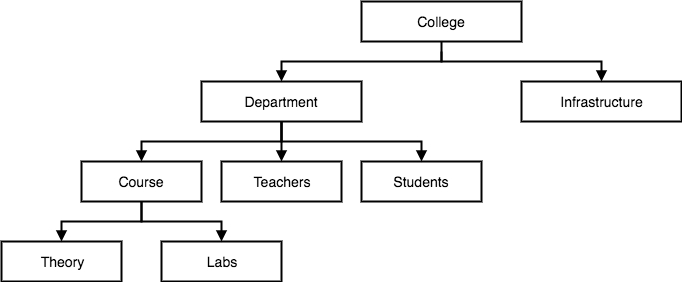
\includegraphics[width=0.5\textwidth]{hierarchical-dbms-model}
	\caption{e.g.: Hierarchical-dbms-model}
	\end{figure}


		\item \textbf{Network Database Systems}
	\begin{itemize}
		\item deals mostly in Many-to-Many relationships, which makes it more complicated and intricated than other DBMS
		\item Network Databases can be accessed by the user in a variety of ways, because the data is arranged in a graphical format
		\item While the Database is structured to be a M-to-M relationship, a child can have more than one parent and vise versa. 
		\item Popular Network Database Systems: Integrated Database Management System(IDMS), Raima Database Manager, TurboIMAGE, Integrated Data Store (IDS) and Univac DMS-1100.
	\end{itemize}
	
							%%% Insert Network Database System Picture %%%	
	\begin{figure}[h]
		\centering
		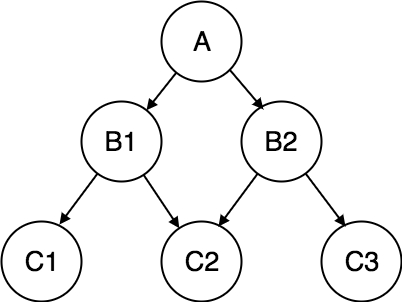
\includegraphics[width=0.2\textwidth]{network-dbms-model}
		\caption{e.g.: Network-dbms-model}
	\end{figure}
	
	\item \textbf{Relational Database Systems}
	\begin{itemize}
		\item A relational Database System is one of the most extensive and complicated systems
		\item It allows the programmers to organize information in a table structure
		\item Connections between the tables are made with "Select" and "Join" operations
		\item 
	\end{itemize}		
	
\end{itemize}
\end{enumerate}




%%% TAST 4 %%%

\section*{Task 4: Entity Relationship Model - Basics}
\begin{enumerate}
\item What are the basic building blocks of the ER model?

\item How are attributes classified in the ER model?

\item What is the significance of cardinality ratios in relationships within the ER model?
\end{enumerate}


%%% TASK 5 %%%

\section*{Task 5: Entity Relationship Model I}
Model the facts below as an Entity Relationship Model using the notation taught in the lecture (Chen notation):

\begin{enumerate}
\item An author has a name, an institution and an email address.

\begin{figure}[h]
\centering
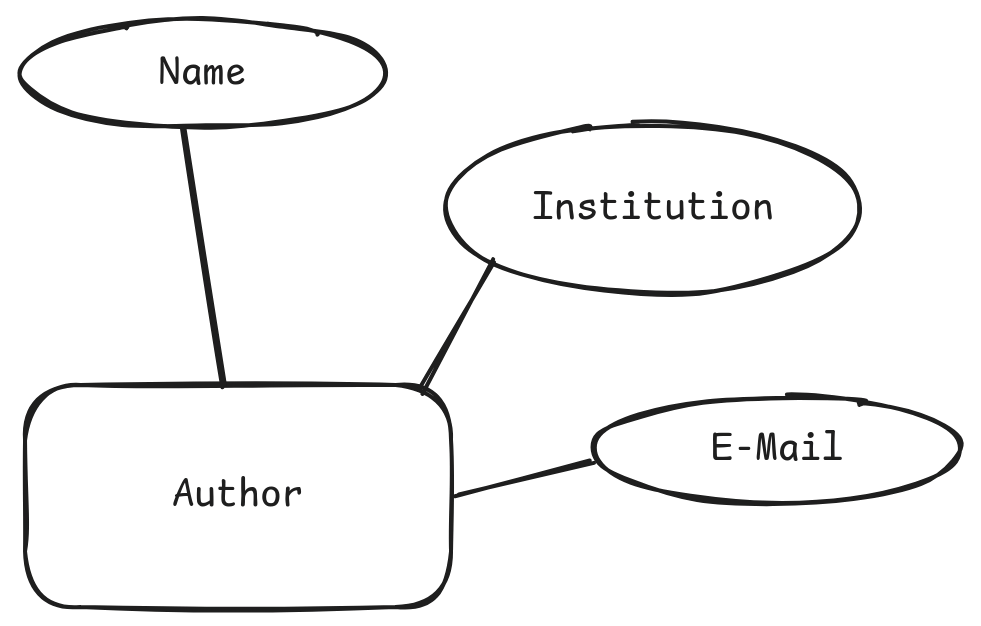
\includegraphics[width=0.3\textwidth]{5.1.png}
\end{figure}

\item An article has a title, three keywords, an abstract, and a DOI(Document Object Identifier).
\begin{figure}[h]
\centering
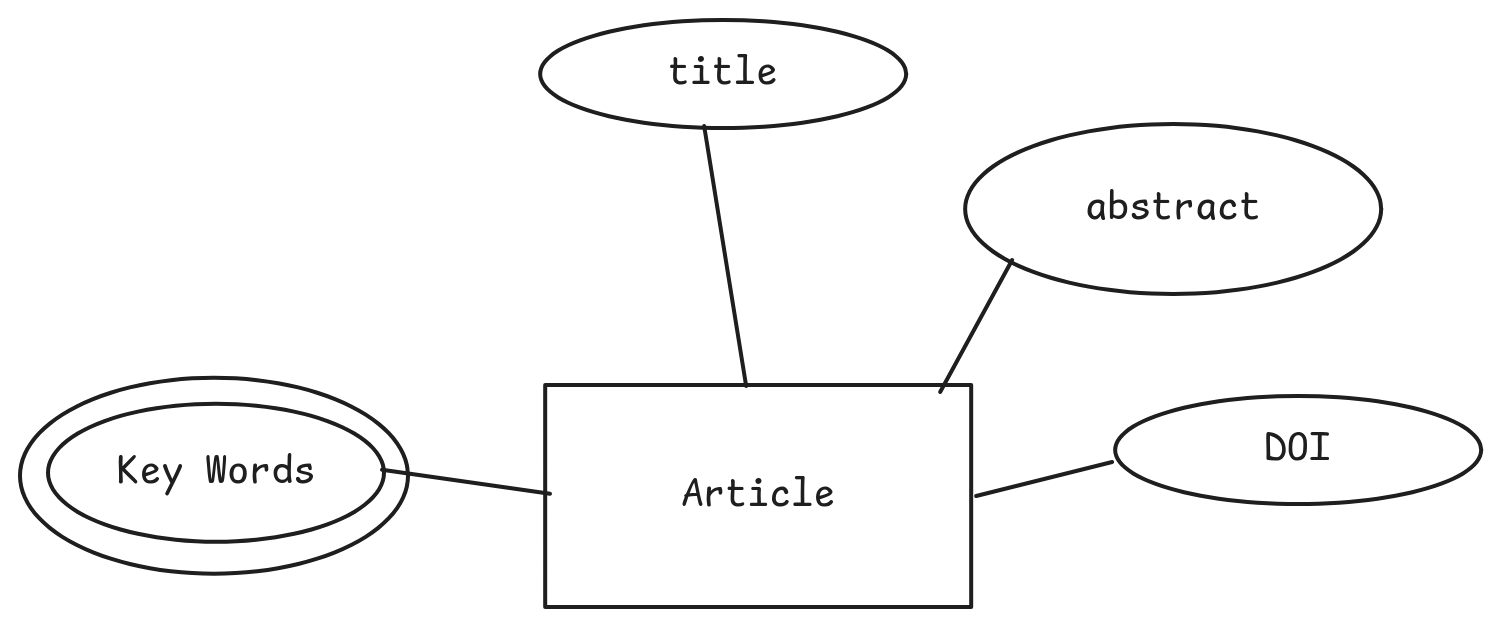
\includegraphics[width=0.4\textwidth]{5.2.png}
\end{figure}

\item Articles are written by multiple authors, and one author may be involved in multiple articles.
\begin{figure}[h]
\centering
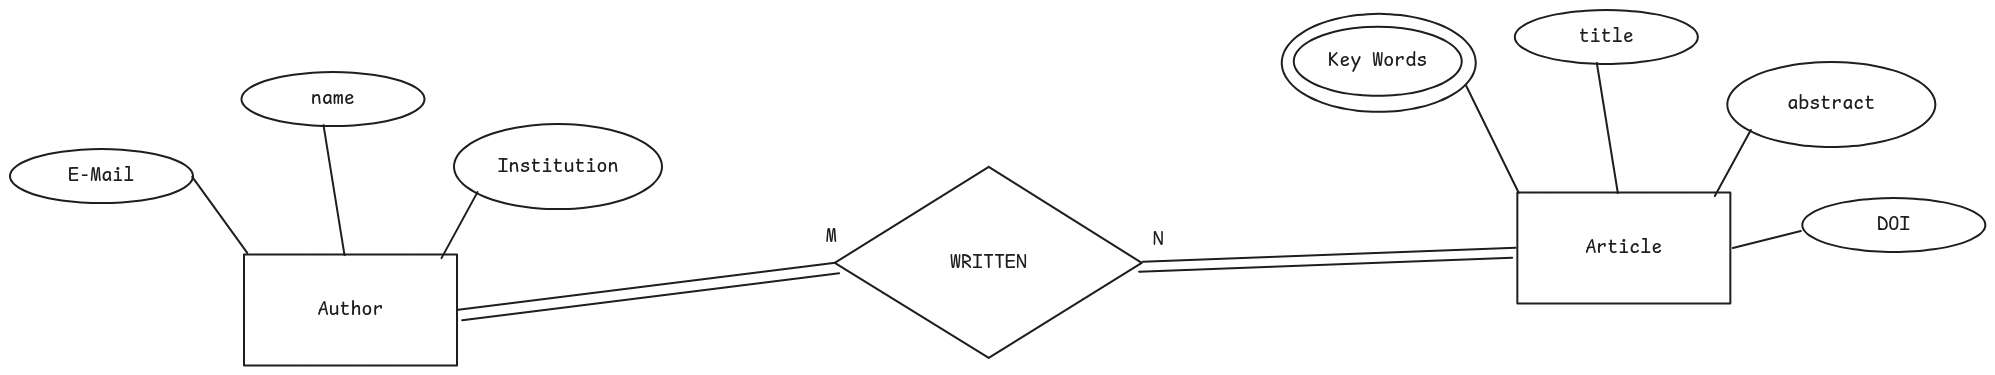
\includegraphics[width=1\textwidth]{5.3.png}
\end{figure}
\end{enumerate}


%%% TASK 6 %%%
\newpage

\section*{Task 6: Entity Relationship Model II}

\begin{enumerate}
\item A publisher has a unique name

\begin{figure}[h]
\centering
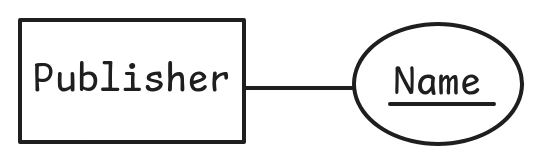
\includegraphics[width=0.3\textwidth]{6.1.png}
\end{figure}

\item A scientist can be an author or a reviewer. Scientists have a name and an e-mail address.
Authors additionally have an institution.

\item Publishers employ reviewers for up to six months to review authors’ articles.

\item An article has a title and a DOI (Document Object Identifier) and is assigned to at least one
reviewer for review.

\item Publishers release articles after reviewing them in a given year.
\end{enumerate}


%%% TASK 7 %%%

\section*{Task 7: Entity Relationship Model III}
\begin{enumerate}
\item An author has a name, an institution and an email address.

\item An article has a title, three keywords, an abstract, and a DOI (Document Object Identifier).

\item A journal has a unique name and topic.

\item Articles are written by multiple authors, and one author may be involved in multiple articles.

\item Authors publish articles in a given year in a journal, and no more than 10 publications by
the same author are ever published in a journal.

\item If articles do not fit the theme of the journal, they will not be published in that journal.
\end{enumerate}


%%% Literaturverzeichnis
\printbibliography

\end{document}